\chapter{Concepts \& Trade-Off}
\setlength{\parindent}{15pt}
\label{ch:conc_trad}
In this section, an overview will be given of how the concept analysed in the preliminary design (the Winged Quadcopter) was chosen.


\section{Concepts Generation}
\label{sec:conc_gene}
In a previous phase of the project, concepts were generated through a brainstorm session and a design option tree \cite{projplan}. From this, five concepts were chosen to be analysed further in order to obtain one concept on which the final design is based. This was done based on feasibility calculations and selecting the designs that seemed most promising. 


The five concepts are: a tailsitter, a tiltable wing in tandem configuration, a Prandtl boxed wing with tiltable propellers, a `tiltrotor' configuration where the propellers (located at the wing tips) can rotate, and a winged quadcopter layout. Detailed information about these concepts can be found in the baseline report \cite{baseline}. All of these concepts have their own strengths and weaknesses. A trade-off was first performed, as elaborated on in \autoref{sec:trad} and in the midterm report \cite{midterm}. The best-performing concept was carried to the final design phase. The concept consists of the outcome of the trade-off combined with some aspects of the other concepts.

\paragraph{Final Concept}
The final concept layout that was chosen was the Winged Quadcopter. It consists of a fuselage with one wing and a tail. On both sides, tiltable propeller engines are installed on the front and aft sides of the wing. This allows the UAV to fly both like a quadcopter and like an airplane. In the initial design, the entire payload module could be taken out of the payload bay. However, it was decided to slightly adapt the mounting mechanism in the final design, such that individual segments of the payload can be taken out separately.


\section{Trade-Off}
\label{sec:trad}
%Trade-off & Sensitivity


% This section can be a lot shorter, by summarising things and refering to the midterm for detailed explanation.
The trade-off performed to determine which concept should be further developed in the the current final phase of the project will be presented here. This section is a summary of the trade-off process performed in the midterm report \cite{midterm}. The trade criteria and their corresponding weights will be discussed in \autoref{sec:trad_crit_weig}, followed by the actual trade-off in \autoref{sec:fina_trad}. Finally, the sensitivity analysis will be presented in \autoref{sec:sens_anal}.

\subsection{Trade Criteria \& Weights}
\label{sec:trad_crit_weig}

The trade criteria have an important impact on the end results of the trade-off. Choosing a criterion which shows no difference in grade for the concepts will adversely impact the trade-off because it will average the results and decrease diversity. This diversity is what should be aimed for to see a distinct difference between the final grades of the concepts, so that the choice for the final concept will be clearer. The explanation of how each criterion affects each concept, and the score achieved by each concept can be found in the midterm report \cite{midterm}. Each concept can score between 0 (bad) and 100 (good).

The first criterion is the performance of the concepts. This criterion has been chosen because there are a lot of requirements on the performance of the aircraft. For this criterion the following elements are examined: the mass, the geometric properties, the endurance, the range, and the power required of each concept. The next criterion is the manoeuvrability and stability where a sub-trade-off was performed using the manoeuvrability, stability, and control of each concept as criteria. Next, the concepts were analysed it terms of ground handling, taking into account how the concepts can be handled during pre- and post-flight procedures. The fourth criterion is the development risk. This criterion was not split into sub-criteria. It inspected the feasibility, complexity and the available knowledge of the concepts, to assess the risk associated with the development phase. The next criterion is the production cost. This criterion is split into manufacturing costs, material costs, mechanisms costs, power and propulsion costs, and finally cost due to weight influence. This criterion has been chosen due to the set limit of 30k EUR for the production cost, limiting the design possibilities for the aircraft. The sustainability criterion is also taken into account and was split into a manufacturing and noise emission analysis. Finally, the reliability criterion took into account the reliability of the propulsion subsystem, the control surfaces, and the wing subsystem.

Assigning weights to the criteria influences the final grades of the trade-off. If a less significant criterion is weighed more than an important criterion, the results will be misleading and the final results might change drastically. Furthermore, it is possible to get biased weights when only one person is responsible for weighing the criteria. Therefore, each member of the team was tasked with filling out a form comparing each criterion to all the other ones. The averages of the weights for each criterion were taken. These averages were normalised to ten and converted into percentages to use for the trade-off. 


\subsection{Final Trade-Off}
\label{sec:fina_trad}

This section will present the results of the final trade-off, which can be seen in \autoref{tab:finaltradeoff}. The outcomes of the trade-off will be briefly discussed to get a grasp as to why the concepts scored as they did. Detailed explanation of the separate criteria scores are the result of extensive research on each criterion. The reasoning behind these scores can be found in the midterm report \cite{midterm}. For clarity, the table contains colours to give an overview of the severity of the scores. Five colours have been used in a 30-15-10-15-30 spacing (Red, Orange, Yellow, Light Green, Dark Green). This spacing has been used to show more detail around the average than around the extremes. In the event that the table cannot be viewed in colour, each score has a superscript showing which category it scores: 1 = Red, 2 = Orange, 3 = Yellow, 4 = Light Green, 5 = Dark Green. 

\begin{table}[H]
    \setlength\extrarowheight{5pt}
    \setlength\arrayrulewidth{1pt}
    \centering
    \caption{Final Trade-Off}
    \label{tab:finaltradeoff}
    \begin{tabular}{r|>{\centering}p{2.1cm}|>{\centering}p{1.9cm}|>{\centering}p{1.3cm}|>{\centering}p{1.1cm}|>{\centering}p{0.8cm}|>{\centering}p{0.7cm}|>{\centering}p{0.4cm}|c} 
    \textbf{Concept \rotatebox{90}{\hspace{0.5cm}Criterion}}        & 
    \rotatebox{90}{\textbf{Performance}}                            &
    \rotatebox{90}{\textbf{M\&S}}                                   & 
    \rotatebox{90}{\textbf{Reliability}}                            & 
    \rotatebox{90}{\textbf{Production Cost}}                        & 
    \rotatebox{90}{\textbf{Development Risk}}                       &
    \rotatebox{90}{\textbf{Sustainability}}                         &
    \rotatebox{90}{\textbf{Ground Handling}}                        &
    \rotatebox{90}{\textbf{Outcome}}
    \\\hline
    Tailsitter      &
    \cellcolor[HTML]{FFFF00}50$^{^3}$ &
    \cellcolor[HTML]{FFFF00}46$^{^3}$ &
    \cellcolor[HTML]{FFFF00}50$^{^3}$ &
    \cellcolor[HTML]{FFFF00}50$^{^3}$ &
    \cellcolor[HTML]{00B050}75$^{^5}$ &
    \cellcolor[HTML]{00B050}84$^{^5}$ &
    \cellcolor[HTML]{92D050}59$^{^4}$ &
    \cellcolor[HTML]{FFFF00}\textbf{55$^{^3}$}
    \\[5pt]\hline
    Tandem          &
    \cellcolor[HTML]{FF0000}17$^{^1}$ &
    \cellcolor[HTML]{FFC000}41$^{^2}$ &
    \cellcolor[HTML]{FFC000}43$^{^2}$ &
    \cellcolor[HTML]{FFC000}35$^{^2}$ &
    \cellcolor[HTML]{FFC000}35$^{^2}$ &
    \cellcolor[HTML]{FF0000}25$^{^1}$ &
    \cellcolor[HTML]{FFC000}38$^{^2}$ &
    \cellcolor[HTML]{FFC000}\textbf{33$^{^2}$}
    \\[5pt]\hline
    Prandtl Box     &
    \cellcolor[HTML]{92D050}67$^{^4}$ &
    \cellcolor[HTML]{FFC000}41$^{^2}$ &
    \cellcolor[HTML]{92D050}68$^{^4}$ &
    \cellcolor[HTML]{FFFF00}50$^{^3}$ &
    \cellcolor[HTML]{92D050}70$^{^4}$ &
    \cellcolor[HTML]{92D050}58$^{^4}$ &
    \cellcolor[HTML]{FFFF00}54$^{^3}$ &
    \cellcolor[HTML]{92D050}\textbf{58$^{^4}$}
    \\[5pt]\hline
    Tiltrotor       &
    \cellcolor[HTML]{FF0000}17$^{^1}$ &
    \cellcolor[HTML]{00B050}73$^{^5}$ &
    \cellcolor[HTML]{92D050}66$^{^4}$ &
    \cellcolor[HTML]{FF0000}25$^{^1}$ &
    \cellcolor[HTML]{FFC000}45$^{^2}$ &
    \cellcolor[HTML]{FF0000}17$^{^1}$ &
    \cellcolor[HTML]{FFFF00}51$^{^3}$ &
    \cellcolor[HTML]{FFC000}\textbf{42$^{^2}$}
    \\[5pt]\hline
    Winged Quad.    &
    \cellcolor[HTML]{00B050}83$^{^5}$ &
    \cellcolor[HTML]{00B050}85$^{^5}$ &
    \cellcolor[HTML]{00B050}84$^{^5}$ &
    \cellcolor[HTML]{FFFF00}55$^{^3}$ &
    \cellcolor[HTML]{00B050}95$^{^5}$ &
    \cellcolor[HTML]{00B050}84$^{^5}$ &
    \cellcolor[HTML]{00B050}82$^{^5}$ &
    \cellcolor[HTML]{00B050}\textbf{81$^{^5}$} 
    \\[5pt] \hline\hline
    Weight          &
    24              &
    22              &
    16              &
    14              &
    11              &
    8               &
    5               &
    \\[5pt]
    \end{tabular}
\end{table}

The best performing concept according to the trade-off is the Winged Quadcopter as it scores best in all criteria.

\subsection{Sensitivity Analysis}
\label{sec:sens_anal}

The goal of the sensitivity analysis is to determine to what extent the final concept selection depends on a change in the weighting of the trade criteria. It alerts whether the chosen concept greatly outperforms all other concepts in one area whilst being poor in the remaining areas. Therefore it is desirable that during the sensitivity analysis the ranking of the concepts do not change. More so, the concept performing best initially, should remain ranked highest at the end of the analysis.

The sensitivity analysis is carried out by successively increasing the weighting of one of the trade criteria, and recalculating the relative score between the concepts. In order to ensure that the analysis is somewhat reliable, the change in weighting should not be too small. An increase of 20\% in the weighting of one criteria yields such results.

\autoref{fig:sensitivityanal} presents a comparison between the scores of the concept corresponding to the changed trade criteria weightings, starting with the original setup. The horizontal axis indicates the type of modified weighting used to achieve the corresponding scores of the concepts. These are the original (normal) weighting and weightings with one criteria increased by 20\%. The score of each concept is shown on the vertical axis.

\begin{figure}[htb]
    \centering
    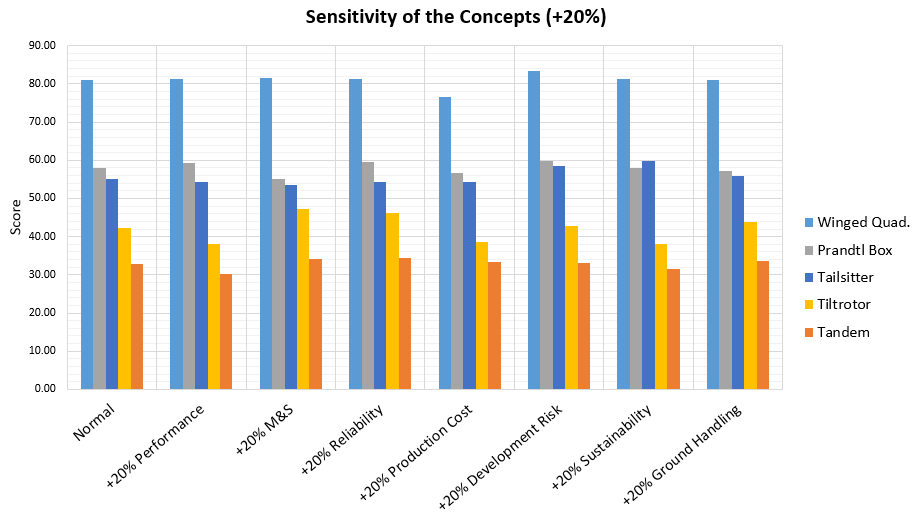
\includegraphics[width=\textwidth]{ConceptTradeOff/Figures/sensitivity}
    \caption{Sensitivity Analysis of the Final Trade-Off}
    \label{fig:sensitivityanal}
\end{figure}

The figure shows that even though the weights of the criteria are changed, The Wing Quadcopter scores highest every time. The gap between the first best and second best does not decrease drastically during the sensitivity analysis, showing that the weighting will not influence the end results. The overall rankings of the concepts also remain unchanged everywhere except when sustainability is weighted 20\% more, this is because the Tailsitter scores 26 higher than the Prandtl Box for that criterion.

Since the Winged Quadcopter greatly outperforms all other concepts throughout the entire sensitivity analysis, it is safe to say that this concept has the greatest potential to satisfy all requirements. Therefore it is sensible to further develop this concept into the preliminary design phase.


\section{Concept Risk Analysis}%Stephanie
\label{sec:conc_anal}
%Technical Risk Assessment



Having selected the Winged Quadcopter configuration, it is possible to asses the potential dangers of not meeting the requirements with this concept. These risks are then mitigated, to ensure the concept can be developed as intended.

Not all requirements are investigated here. Some were deemed not relevant enough for the risk analysis, while others were found to be met naturally. Further explanation of these choices can be found in the midterm report \cite{midterm}. Only the crucial requirements posing a risk larger than 4, and the ones that have changed since the preliminary design phase, are elaborated on here. This can be seen in \autoref{tab:over_tech_risk}, where the likelihood of occurrence (L) and impact (I) are marked between 1 (impossible or negligible) and 4 (very likely or catastrophic). The product of these forms the risk (R).  All requirement codes can be found in \autoref{sec:requ}. After investigating the risks, they are mapped in \autoref{tab:risk_map_wing_quad}; here the SYS- proposition was left out for clarity. Mitigation measures have been taken for all the requirements with a risk score of 4 and higher. These can also be found in \autoref{tab:over_tech_risk}, where L, I and R have the same meaning, but now applied to the mitigated risk. 
%Some of the risks that were left out in the midterm report are included now --- maybe something about cost


\begin{table}[ht]
    \centering
    \caption{Overview of Applicable Technical Risks and Mitigation Measures}
    \label{tab:over_tech_risk}
    \begin{tabularx}{\textwidth}{>{\small}l L *{3}{>{\small}c} }
    \toprule
    \bfseries Requirement &\bfseries Impact and likeliness explanation &\bfseries L &\bfseries I &\bfseries R
    \\ \midrule
    %Maybe also include cost....
    SYS-PH-1.1  & The wingspan is 2.92 m, which means it can not fit in a van as a whole. However, it is possible to dismantle the wings, which solves the problem.    & 1 & 3 & 3
    \\ \hdashline
    SYS-PF-1.1  & The 10 kg requirement can be met, however, when maximum range or endurance is desired, part of this payload should consist of batteries.               & 2 & 2 & 4
    \\ \hdashline
    SYS-PF-1.2  & When the UAV does not reach a maximum velocity of 200 km/h it will perform less in missions where endurance is the driving factor.     & 3 & 2 & 6
    \\ \hdashline
    SYS-PF-1.3R  & Since the payload can carry extra batteries, it will be possible to meet this requirement. & 1 & 3 & 3
    \\ \hdashline 
    SYS-PF-2.3   & Hovering is one of the most power-intensive flight phases, and therefore this severely reduces the endurance.          & 2 & 3 & 6
    \\ \toprule
    \bfseries Requirement & \bfseries Mitigation measure   & \bfseries L &\bfseries I &\bfseries R
    \\ \midrule
    SYS-PF-1.2  & When the maximum velocity that is designed for is 200 km/h, the maximum attainable velocity will still approach this. Therefore, the impact is decreased.         & 3 & 1 & 3
    \\ \hdashline
    SYS-PF-2.3 & The payload mounting mechanism will be designed such that the UAV is able to release it within one minute. Therefore less hovering time is required.             & 2 & 1 & 2
    \\ \bottomrule
    \end{tabularx}
\end{table}

\begin{table}[H]
    \centering
    \caption{Risk Map of the Winged Quadcopter Before Mitigation}
    \label{tab:risk_map_wing_quad}
    \begin{tabular}{  p{2.2cm}  p{3.2cm}    p{2.95cm}   p{2.8cm}    p{2.4cm}    }
    \toprule
                    & (Almost) impossible                                       & Improbable                                    & Probable                          & Very likely
    \\ \midrule
    Catastrophic    &\cellcolor[HTML]{d9ead3}                                   &\cellcolor[HTML]{fff2cc}                       &\cellcolor[HTML]{f4cccc}           &\cellcolor[HTML]{f4cccc}
    \\ \hdashline
    Critical        &\cellcolor[HTML]{d9ead3} PH-1.1, PF-1.3R    &\cellcolor[HTML]{fff2cc} PF-2.3 &\cellcolor[HTML]{fff2cc}           &\cellcolor[HTML]{f4cccc}
    \\ \hdashline
    Marginal        &\cellcolor[HTML]{d9ead3}                      &\cellcolor[HTML]{d9ead3}  PF-1.1                &\cellcolor[HTML]{fff2cc} PF-1.2    &\cellcolor[HTML]{fff2cc}
    \\ \hdashline
    Negligible      &\cellcolor[HTML]{d9ead3}                                   &\cellcolor[HTML]{d9ead3}                       &\cellcolor[HTML]{d9ead3}           &\cellcolor[HTML]{d9ead3}
    \\ \bottomrule
    \end{tabular}
\end{table}




